\documentclass[ignorenonframetext,]{beamer}
\usepackage{amssymb,amsmath}
\usepackage{ifxetex,ifluatex}
\usepackage{fixltx2e} % provides \textsubscript
\usepackage{lmodern}
\ifxetex
  \usepackage{fontspec,xltxtra,xunicode}
  \defaultfontfeatures{Mapping=tex-text,Scale=MatchLowercase}
  \newcommand{\euro}{€}
\else
  \ifluatex
    \usepackage{fontspec}
    \defaultfontfeatures{Mapping=tex-text,Scale=MatchLowercase}
    \newcommand{\euro}{€}
  \else
    \usepackage[T1]{fontenc}
    \usepackage[utf8]{inputenc}
      \fi
\fi
\IfFileExists{upquote.sty}{\usepackage{upquote}}{}
% use microtype if available
\IfFileExists{microtype.sty}{\usepackage{microtype}}{}
\usepackage{color}
\usepackage{fancyvrb}
\newcommand{\VerbBar}{|}
\newcommand{\VERB}{\Verb[commandchars=\\\{\}]}
\DefineVerbatimEnvironment{Highlighting}{Verbatim}{commandchars=\\\{\}}
% Add ',fontsize=\small' for more characters per line
\usepackage{framed}
\definecolor{shadecolor}{RGB}{248,248,248}
\newenvironment{Shaded}{\begin{snugshade}}{\end{snugshade}}
\newcommand{\KeywordTok}[1]{\textcolor[rgb]{0.13,0.29,0.53}{\textbf{{#1}}}}
\newcommand{\DataTypeTok}[1]{\textcolor[rgb]{0.13,0.29,0.53}{{#1}}}
\newcommand{\DecValTok}[1]{\textcolor[rgb]{0.00,0.00,0.81}{{#1}}}
\newcommand{\BaseNTok}[1]{\textcolor[rgb]{0.00,0.00,0.81}{{#1}}}
\newcommand{\FloatTok}[1]{\textcolor[rgb]{0.00,0.00,0.81}{{#1}}}
\newcommand{\CharTok}[1]{\textcolor[rgb]{0.31,0.60,0.02}{{#1}}}
\newcommand{\StringTok}[1]{\textcolor[rgb]{0.31,0.60,0.02}{{#1}}}
\newcommand{\CommentTok}[1]{\textcolor[rgb]{0.56,0.35,0.01}{\textit{{#1}}}}
\newcommand{\OtherTok}[1]{\textcolor[rgb]{0.56,0.35,0.01}{{#1}}}
\newcommand{\AlertTok}[1]{\textcolor[rgb]{0.94,0.16,0.16}{{#1}}}
\newcommand{\FunctionTok}[1]{\textcolor[rgb]{0.00,0.00,0.00}{{#1}}}
\newcommand{\RegionMarkerTok}[1]{{#1}}
\newcommand{\ErrorTok}[1]{\textbf{{#1}}}
\newcommand{\NormalTok}[1]{{#1}}
\usepackage{longtable,booktabs}
\usepackage{caption}
% These lines are needed to make table captions work with longtable:
\makeatletter
\def\fnum@table{\tablename~\thetable}
\makeatother
\usepackage{letltxmacro}
\makeatletter
\def\maxwidth{\ifdim\Gin@nat@width>\linewidth\linewidth\else\Gin@nat@width\fi}
\def\maxheight{\ifdim\Gin@nat@height>\textheight0.8\textheight\else\Gin@nat@height\fi}
\makeatother
\AtBeginDocument{
  \LetLtxMacro\Oldincludegraphics\includegraphics
  \renewcommand{\includegraphics}[2][]{%
    \Oldincludegraphics[#1,width=\maxwidth,height=\maxheight,keepaspectratio]{#2}}
}

% Comment these out if you don't want a slide with just the
% part/section/subsection/subsubsection title:
\AtBeginPart{
  \let\insertpartnumber\relax
  \let\partname\relax
  \frame{\partpage}
}
\AtBeginSection{
  \let\insertsectionnumber\relax
  \let\sectionname\relax
  \frame{\sectionpage}
}
\AtBeginSubsection{
  \let\insertsubsectionnumber\relax
  \let\subsectionname\relax
  \frame{\subsectionpage}
}

\setlength{\parindent}{0pt}
\setlength{\parskip}{6pt plus 2pt minus 1pt}
\setlength{\emergencystretch}{3em}  % prevent overfull lines
\setcounter{secnumdepth}{0}
\usepackage[utf8]{inputenc}
\usepackage[russian]{babel}

\title{Эконометрика. Лекция 1}

\begin{document}
\frame{\titlepage}

\begin{frame}{Эконометрика на одном слайде :)}

\begin{block}{Вопросы:}

\begin{itemize}
\itemsep1pt\parskip0pt\parsep0pt
\item
  Как устроен мир? Как переменная $x$ влияет на переменную $y$?
\item
  Что будет завтра? Как спрогнозировать переменную $y$?
\end{itemize}

\end{block}

\begin{block}{Ответ:}

Модель --- формула для объясняемой переменной

\end{block}

\begin{block}{Например:}

\begin{itemize}
\itemsep1pt\parskip0pt\parsep0pt
\item
  $y_i=\beta_1+\beta_2 x_i + \varepsilon_i$
\item
  $y_{t}=y_{t-1}+\varepsilon_t$
\end{itemize}

\end{block}

\end{frame}

\begin{frame}{Данные:}

\begin{itemize}
\itemsep1pt\parskip0pt\parsep0pt
\item
  Одна зависимая, объясняемая, переменная: $y$
\item
  Несколько независимых, объясняющих, переменных: $x$, $z$, $\ldots$
\item
  По каждой переменной $n$ наблюдений: $y_1$, $y_2$, $\ldots$, $y_n$
\end{itemize}

\begin{longtable}[c]{@{}rr@{}}
\toprule\addlinespace
Длина тормозного пути (м), $y_i$ & Скорость машины (км/ч), $x_i$
\\\addlinespace
\midrule\endhead
0.6 & 6.68
\\\addlinespace
3.0 & 6.68
\\\addlinespace
1.2 & 11.69
\\\addlinespace
\ldots{} & \ldots{}
\\\addlinespace
\bottomrule
\end{longtable}

Исторические данные 1920-х годов :)

\end{frame}

\begin{frame}{Всегда изображайте данные!}

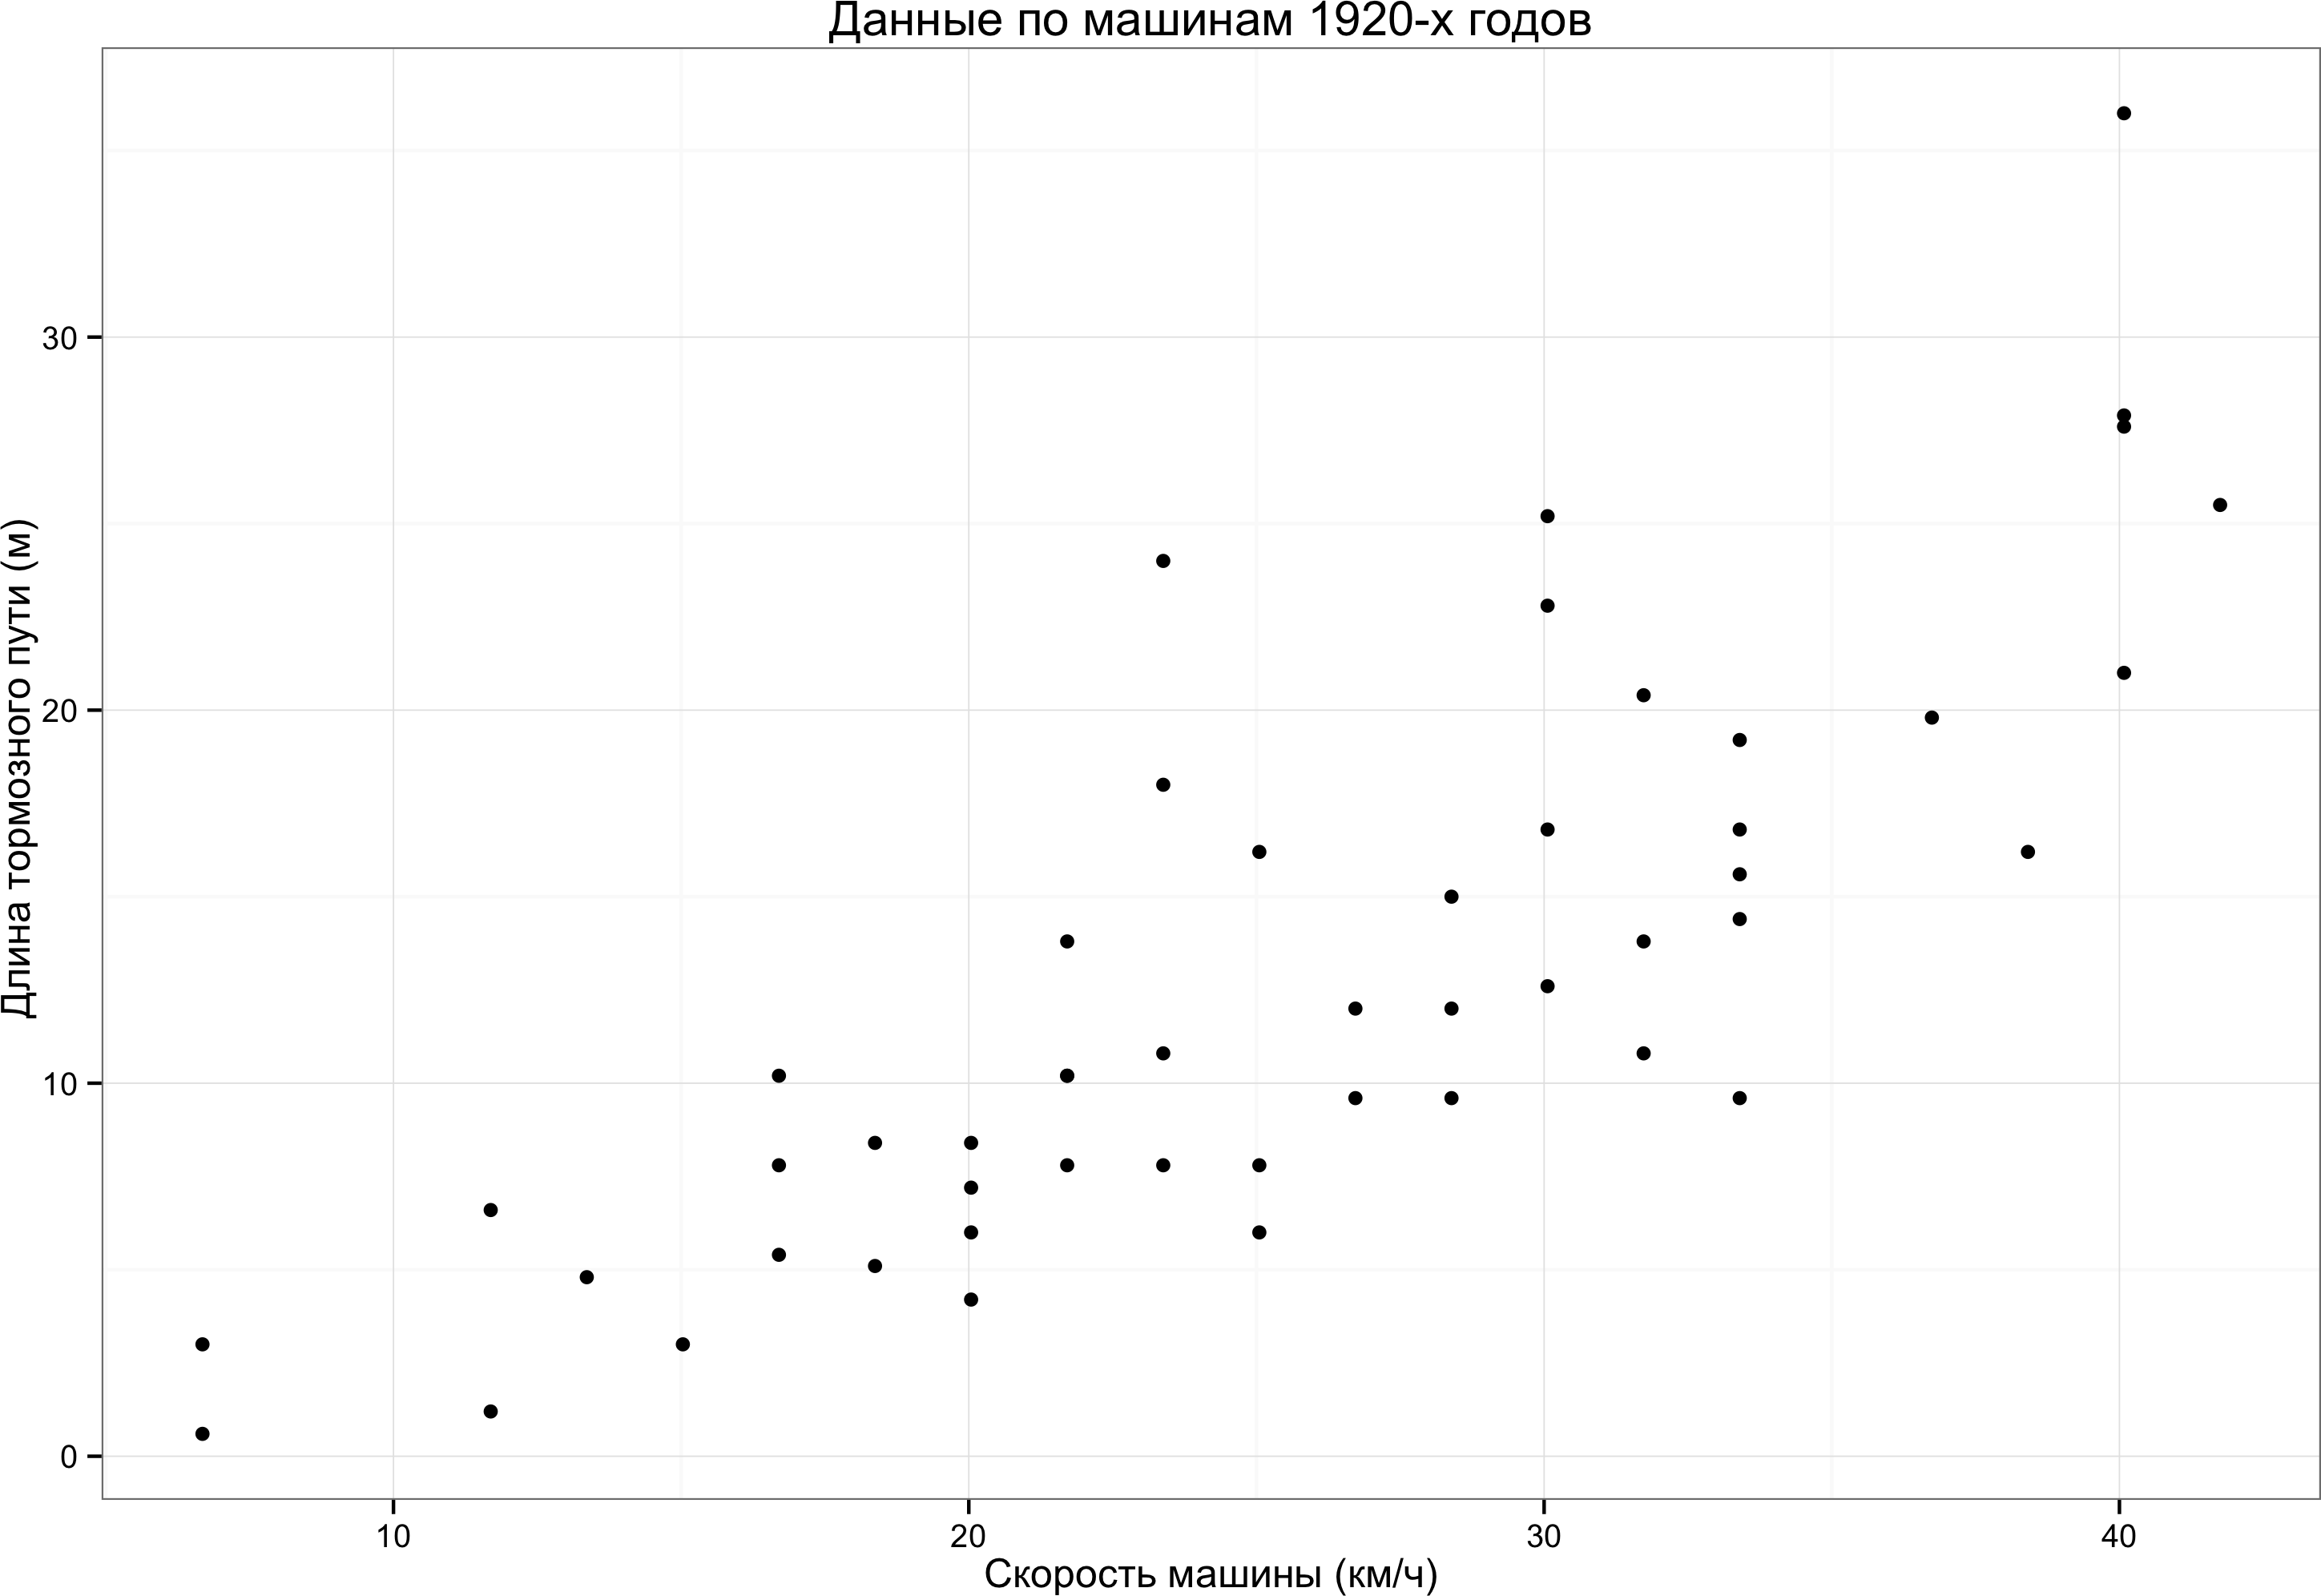
\includegraphics{./lec_01_files/figure-beamer/unnamed-chunk-3.png}

\end{frame}

\begin{frame}{Модель:}

Пример: $y_i=\beta_1 + \beta_2 x_i + \varepsilon_i$

\begin{itemize}
\itemsep1pt\parskip0pt\parsep0pt
\item
  Наблюдаемые переменные: $y$, $x$
\item
  Неизвестные параметры: $\beta_2$, $\beta_2$
\item
  Случайная составляющая, ошибка: $\varepsilon$
\end{itemize}

\begin{block}{План действий}

\begin{itemize}
\itemsep1pt\parskip0pt\parsep0pt
\item
  придумать адекватную модель
\item
  получить оценки неизвестных параметров: $\hat{\beta}_1$,
  $\hat{\beta}_2$
\item
  прогнозировать, заменив неизвестные параметры на оценки: \[
  \hat{y}_i=\hat{\beta}_1 + \hat{\beta}_2 x_i
  \]
\end{itemize}

\end{block}

\end{frame}

\begin{frame}{Метод наименьших квадратов}

\begin{itemize}
\itemsep1pt\parskip0pt\parsep0pt
\item
  Способ получить оценки неизвестных параметров модели исходя из
  реальных данных.
\end{itemize}

Ошибка прогноза: $e_i=y_i-\hat{y}_i$.

Сумма квадратов ошибок прогноза: \[
Q(\hat{\beta}_1,\hat{\beta}_2)=\sum_{i=1}^n e_i^2=\sum_{i=1}^n (y_i-\hat{y}_i)^2
\]

Суть МНК: В качестве оценок взять такие $\hat{\beta}_1$,
$\hat{\beta}_2$, при которых сумма квадратов ошибок прогноза, $Q$,
минимальна.

\end{frame}

\begin{frame}{Пример с машинами:}

Фактические данные:

$x_1=6.68$, $x_2=6.68$, \ldots{},

$y_1=0.6$, $y_2=3$, \ldots{}

Модель: $y_i=\beta_1+\beta_2 x_i+\varepsilon_i$. Формула для прогнозов:
$\hat{y}_i=\hat{\beta}_1 + \hat{\beta}_2 x_i$

Сумма квадратов ошибок прогнозов: $Q=\sum_{i=1}^n (y_i-\hat{y}_i)^2$

\[
Q=(0.6-\hat{\beta}_1-\hat{\beta}_2 6.68)^2+(3-\hat{\beta}_1-\hat{\beta}_2 6.68)^2+...
\]

Точка минимума, найдена в R: $\hat{\beta}_1=-5.3$, $\hat{\beta}_2=0.7$:

Формула для прогнозов: $\hat{y}_i=-5.3 + 0.7 x_i$

\end{frame}

\begin{frame}{Простой пример}

\begin{longtable}[c]{@{}rrr@{}}
\toprule\addlinespace
Имя & Вес (кг), $y_i$ & Рост (см), $x_i$
\\\addlinespace
\midrule\endhead
Вася & 60 & 170
\\\addlinespace
Коля & 70 & 170
\\\addlinespace
Петя & 80 & 180
\\\addlinespace
\bottomrule
\end{longtable}

Модель: $y_i=\beta x_i +\varepsilon_i$, Прогнозы:
$\hat{y}_i=\hat{\beta}x_i$.

Сумма квадратов ошибок: \[
Q(\hat{\beta})=(60-\hat{\beta}170)^2+(70-\hat{\beta}170)^2+(80-\hat{\beta}180)^2
\]

\end{frame}

\begin{frame}{Решение задачи минимизации}

Сумма квадратов ошибок: \[
Q(\hat{\beta})=(60-\hat{\beta}170)^2+(70-\hat{\beta}170)^2+(80-\hat{\beta}180)^2
\]

Производная:

\begin{multline}
Q'(\hat{\beta})=-2\cdot 170\cdot (60-\hat{\beta}170)-2\cdot 170\cdot(70-\hat{\beta}170)\\
-2\cdot 180\cdot(80-\hat{\beta}180)
\end{multline}

Приравняв производную к нулю получаем: \[
\hat{\beta}=0.4047
\]

\end{frame}

\begin{frame}{Терминология и обозначения:}

$y_i$ --- зависимая, объясняемая, переменная

$x_i$ --- регрессор, объясняющая переменная

$\varepsilon_i$ --- ошибка, ошибка модели, случайная составляющая

$\hat{y}_i$ --- прогноз, прогнозное значение

$e_i=y_i-\hat{y}_i$ --- остаток, ошибка прогноза

$RSS=\sum_{i=1}^n e_i^2$ --- сумма квадратов остатков

\end{frame}

\begin{frame}{Три простых случая в явном виде}

\begin{block}{$y_i=\beta+\varepsilon_i$}

\end{block}

\begin{block}{$y_i=\beta x_i+\varepsilon_i$}

\end{block}

\begin{block}{$y_i=\beta_1+\beta_2 x_i+\varepsilon_i$}

\end{block}

\end{frame}

\begin{frame}{Случай $y_i=\beta+\varepsilon_i$. Нет объясняющей
переменной.}

\begin{itemize}
\itemsep1pt\parskip0pt\parsep0pt
\item
  Сколько лет Васе?
\end{itemize}

Анна: 35. Белла: 27. Вика: 34.

Спрогнозируем Васин возраст с помощью МНК!

Наблюдения: $y_1$, $y_2$, \ldots{}, $y_n$

Модель: $y_i=\beta+\varepsilon_i$. Прогнозы: $\hat{y}_i=\hat{\beta}$

Сумма квадратов остатков:
$Q=\sum_{i=1}^n (y_i-\hat{y}_i)^2= \sum_{i=1}^n(y_i-\hat{\beta})^2$

Находим производную: $Q'(\hat{\beta})=\sum_{i=1}^n -2(y_i-\hat{\beta})$

\end{frame}

\begin{frame}{Случай $y_i=\beta+\varepsilon_i$. Решение.}

Упрощаем производную:

\begin{multline}
Q'(\hat{\beta})=\sum_{i=1}^n -2(y_i-\hat{\beta})=-2 \sum_{i=1}^n (y_i-\hat{\beta})=\\
-2 (\sum_{i=1}^n y_i-\sum_{i=1}^n \hat{\beta})=-2(\sum_{i=1}^n y_i-n\hat{\beta})
\end{multline}

Приравняв к нулю получаем: $\sum_{i=1}^n y_i=n\hat{\beta}$ или

$\hat{\beta}=\sum_{i=1}^n y_i /n=(y_1+y_2+...+y_n)/n=\bar{y}$

МНК-прогноз возраста Васи: $\hat{\beta}=(35+27+34)/3=32$

\end{frame}

\begin{frame}{Случай $y_i=\beta x_i+\varepsilon_i$. Пропорциональность.}

\end{frame}

\begin{frame}{Случай \$ \$. Парная регрессия.}

Предварительные замечания:

$\bar{x}=\sum_{i=1}^n x_i$, поэтому:

$n\bar{x}=\sum_{i=1}^n x_i$ или $\sum_{i=1}^n \bar{x}=\sum_{i=1}^n x_i$.

\end{frame}

\begin{frame}{Первая регрессия в R}

(!) Установите R, Rstudio и дополнительные пакеты

Три режима работы с Rstudio:

\begin{itemize}
\item
  диалоговый, консольный
\item
  написание скрипта или программы
\item
  написание документа, ``грамотное программирование''
\end{itemize}

\end{frame}

\begin{frame}{Консольный режим}

\ldots{} тут скринкаст

\end{frame}

\begin{frame}[fragile]{Консольный режим. Резюме\ldots{}}

\begin{itemize}
\itemsep1pt\parskip0pt\parsep0pt
\item
  R отличает заглавные и прописные буквы.
\end{itemize}

\begin{Shaded}
\begin{Highlighting}[]
\NormalTok{a <-}\StringTok{ }\DecValTok{5}
\NormalTok{A <-}\StringTok{ }\DecValTok{4}
\NormalTok{a +}\StringTok{ }\NormalTok{A}
\end{Highlighting}
\end{Shaded}

\begin{verbatim}
## [1] 9
\end{verbatim}

\begin{itemize}
\item
  присваивания \texttt{a \textless{}- 5} и \texttt{a = 5} абсолютно
  равнозначны
\item
  знак \texttt{+} в командной строке означает неоконченную команду

  \begin{itemize}
  \itemsep1pt\parskip0pt\parsep0pt
  \item
    может означать забытую незакрытую скобку
  \item
    избавиться можно нажатием клавиши \texttt{Esc}
  \end{itemize}
\item
  \texttt{tab} облегачает жизнь, дописывая длинные названия
\end{itemize}

\end{frame}

\begin{frame}{Написание скрипта}

(тут скринкаст)

\end{frame}

\begin{frame}[fragile]{Написание скрипта. Резюме\ldots{}}

\begin{itemize}
\item
  \texttt{ctrl+Enter} (\texttt{cmd+Enter} на Маке) исполняет текущую
  строчку или несколько строк
\item
  два основных объекта: вектор и табличка с данными
\end{itemize}

\begin{Shaded}
\begin{Highlighting}[]
\NormalTok{x <-}\StringTok{ }\KeywordTok{c}\NormalTok{(}\DecValTok{5}\NormalTok{,}\DecValTok{2}\NormalTok{,}\DecValTok{1}\NormalTok{)}
\NormalTok{d <-}\StringTok{ }\KeywordTok{data.frame}\NormalTok{(}\DataTypeTok{rost=}\KeywordTok{c}\NormalTok{(}\DecValTok{170}\NormalTok{,}\DecValTok{170}\NormalTok{,}\DecValTok{180}\NormalTok{),}\DataTypeTok{ves=}\KeywordTok{c}\NormalTok{(}\DecValTok{60}\NormalTok{,}\DecValTok{70}\NormalTok{,}\DecValTok{80}\NormalTok{))}
\end{Highlighting}
\end{Shaded}

\begin{itemize}
\itemsep1pt\parskip0pt\parsep0pt
\item
  любой реальный скрипт начинается с загрузки дополнительных пакетов
\end{itemize}

\begin{Shaded}
\begin{Highlighting}[]
\KeywordTok{library}\NormalTok{(}\StringTok{"dplyr"}\NormalTok{)}
\KeywordTok{library}\NormalTok{(}\StringTok{"ggplot2"}\NormalTok{)}
\end{Highlighting}
\end{Shaded}

\end{frame}

\begin{frame}[fragile]{Резюме. Загрузка данных.}

Загрузка данных из электронной таблицы (Excel, Libre Office Calc,
Gnumeric \ldots{})

\begin{enumerate}
\def\labelenumi{\arabic{enumi}.}
\item
  Причесать данные
\item
  Сохранить данные в формате csv
\item
  Прочитать данные в R командой
\end{enumerate}

\begin{Shaded}
\begin{Highlighting}[]
\NormalTok{d <-}\StringTok{ }\KeywordTok{read.table}\NormalTok{(}\StringTok{"mydata.csv"}\NormalTok{)}
\end{Highlighting}
\end{Shaded}

\end{frame}

\begin{frame}{Резюме. Поглядеть на табличку}

Данные в табличке \texttt{d}.

\begin{itemize}
\itemsep1pt\parskip0pt\parsep0pt
\item
  начало и конец таблички: \texttt{head(d)}, \texttt{tail(d)}
\item
  описание таблички: \texttt{str(d)}
\item
  описательные статистики: \texttt{summary(d)}
\item
  достать переменную \texttt{speed} из таблички: \texttt{d\$speed}
\item
  достать вторую строку из таблички: \texttt{d{[}2,{]}}
\item
  достать второй столбец из таблички: \texttt{d{[},2{]}}
\item
  преобразовать или создать новую переменную:
  \texttt{d \textless{}- mutate(d,speed2=speed\^{}2)}
\end{itemize}

\end{frame}

\begin{frame}{Резюме. Два базовых графика}

\begin{itemize}
\item
  Гистограмма
\item
  Диаграмма рассеяния
\item
  Не забывайте подписи!!!
\end{itemize}

\end{frame}

\begin{frame}{Резюме. Простой пример регрессии}

\end{frame}

\begin{frame}{Вопросы}

\begin{itemize}
\item
  А будет ли решение задачи минимизации единственным?
\item
  А будет ли решение задачи минимизации вообще существовать?
\item
  А почему сумма квадратов остатков, а не, скажем, модулей?
\item
  А насколько точны полученные оценки?
\item
  \ldots{}
\end{itemize}

\end{frame}

\begin{frame}[fragile]{Написание документа}

\begin{Shaded}
\begin{Highlighting}[]
\KeywordTok{library}\NormalTok{(}\StringTok{"dplyr"}\NormalTok{)}
\KeywordTok{library}\NormalTok{(}\StringTok{"ggplot2"}\NormalTok{)}
\NormalTok{d <-}\StringTok{ }\NormalTok{cars }
\KeywordTok{head}\NormalTok{(cars)}
\end{Highlighting}
\end{Shaded}

\begin{verbatim}
##   speed dist
## 1     4    2
## 2     4   10
## 3     7    4
## 4     7   22
## 5     8   16
## 6     9   10
\end{verbatim}

\begin{Shaded}
\begin{Highlighting}[]
\CommentTok{# %>% mutate(dist=0.3*dist,speed=1.67*speed)}
\end{Highlighting}
\end{Shaded}

\end{frame}

\begin{frame}

$\bar{y}=(y_1+y_2+...+y_n)/n$ --- среднее значение $y$

$TSS=\sum_{i=1}^n (y_i-\bar{y})^2$ --- общая сумма квадратов

$ESS=\sum_{i=1}^n (\hat{y}_i-\bar{y})^2$ --- объясненная сумма квадратов

\end{frame}

\end{document}
